\documentclass[parskip=full,11pt]{scrartcl}
\usepackage[utf8]{inputenc}
\usepackage[T1]{fontenc}
\usepackage[german]{babel}
\usepackage[useregional]{datetime2}
\usepackage[pdfborderstyle={/S/U/W 0}]{hyperref}
\usepackage[nameinlink]{cleveref}
\usepackage[section]{placeins}
\usepackage{xcolor}
\usepackage{graphicx}
\usepackage{csquotes}
\usepackage{amsmath} % for $\text{}$
\usepackage{pflichtenheft}
\usepackage{enumitem}
\setlist{nosep}

\newcommand\urlpart[2]{$\underbrace{\text{\texttt{#1}}}{\text{#2}}$}
\raggedbottom
\crefname{figure}{Abb}{Abb}

\hypersetup{
	pdftitle={Pflichtenheft},
	bookmarks=true,
}

% section numbers in margins:
\renewcommand\sectionlinesformat[4]{\makebox[0pt][r]{#3}#4}

% header & footer
\usepackage{scrlayer-scrpage}
\lofoot{\today}
\refoot{\today}
\pagestyle{scrheadings}

\newcommand\producttitle{GO-App}

\title{Pflichtenheft: \producttitle}
\author{Lukas Dippon
        \and Jens Kienle
        \and Matthias Noll
        \and Fabian Röpke
        \and Tim Schmidt
        \and Simon Vögele}

\begin{document}
\maketitle
\thispagestyle{empty} % removed page number from title
\newpage
\tableofcontents
\newpage

\section{Einleitung}
Studenten und Mitarbeiter des KIT treffen sich gerne zum gemeinsamen Essen oder Lernen.
Dazu ist an einem bestimmten Tag immer notwendig zu wissen, ob bereits ein Treffen vereinbart wurde.
Am Treffpunkt angekommen, möchte man wissen, an welchem Ort sich die Gruppe befindet, um nicht lange suchen zu müssen.
Unsere App soll es angemeldeten Benutzern ermöglichen, sich in Gruppen zu organisieren.
In den Gruppen kann der Zeit- und Treffpunkt bestimmt werden.
Nach der Festlegung des Treffens soll die App die GPS-Standorte der Mitglieder anzeigen, um das Treffen zu vereinfachen.

%%%%%%%%%%%%%%
\pagebreak
\section{Kriterien}
% Diese Section sollte kurz und knapp "für Manager" sein
% und auf eine Seite passen.

\subsection{Pflichtkriterien}
\criterion{Gruppen}{groups}{10}
Mehrere Nutzer können sich in Gruppen zusammenschließen.
Ein Nutzer kann in beliebig vielen Gruppen Mitglied sein.

\criterion{Eigene Position auf Umgebungskarten}{location}{20}
Der Nutzer ist in der Lage, seine aktuelle Position auf einer Karte der nahen
Umgebung einzusehen.

\criterion{Festlegbare Treffpunkte}{meetingpoints}{30}
Innerhalb von Gruppen können Treffpunkte festgelegt werden,
die den Mitgliedern auf der Karte angezeigt werden.

\criterion{Gegenseitige Ortung}{positions}{40}
Nutzer sind in der Lage, ihre aktuelle Position mit anderen Gruppenmitgliedern
über einen festlegbaren Zeitraum zu teilen.
Diese wird dann allen Gruppenmitgliedern auf der Karte angezeigt und laufend
aktualisiert.

\criterion{Datenschutz}{privacy}{50}
Die Positionsdaten des Nutzers werden nur während des festgelegten Zeitraumes
(\critLink{positions}) gesendet und serverseitig nicht
längerfristig gespeichert.

\criterion{Nutzerkonten}{account}{60}
Ein persönliches Nutzerkonto ermöglicht es Nutzern,
Gruppenzugehörigkeiten und Datenschutzoptionen zu speichern.

\subsection{Kürkriterien}
\criterionOpt{Abstimmungen}{vote}{10}
Innerhalb von Gruppen können die Nutzer über nächste Treffpunkte abstimmen.

\criterionOpt{1 zu 1 Verbindung}{1to1}{20}
Der Positionsaustausch zwischen zwei einzelnen Nutzern außerhalb von Gruppen
soll möglich und besonders einfach sein.

\criterionOpt{Detailliertere Innenraumkarten}{indoor}{30}
Innenräume mit hoher Nutzerdichte bekommen detaillierte Innenraumkarten.

\criterionOpt{Gruppenchat}{chat}{40}
Innerhalb der Gruppen können simple Textnachrichten versendet werden.

\criterionOpt{Eigene Server}{ownServer}{50}
Es ist dem Nutzer möglich, einen eigenen Server zu erstellen und zu verwalten.

\criterionOpt{Server-Wechsel}{switchServer}{60}
Um \critLink{ownServer} ausnutzen zu können, ist es dem Nutzer
möglich, den verwendeten Server zu wechseln.

\criterionOpt{Zeitplan für Positionsübertragung}{timetable}{70}
Der Nutzer kann zu bestimmten Zeiten seine Position automatisch an bestimmte
Gruppen übertragen lassen.

\criterionOpt{Passwortzurücksetzung}{passwordReset}{80}
Der Nutzer kann sein Passwort zurücksetzen lassen, wenn er sich über eine zuvor
festgelegte E-Mail-Adresse authentifizieren kann.

\subsection{Abgrenzungskriterien}
\criterionDemarc{Kein Social Network}{socialNetwork}{10}
Die App bietet keine Plattform um Bilder oder andere persönliche Eindrücke mit
anderen zu teilen.

\criterionDemarc{Kontakt nur zu Freunden}{friendsOnly}{20}
Die App möchte die Kommunikation in bereits bestehenden Gruppen vereinfachen,
nicht den Kontakt zu Fremden ermöglichen.

\criterionDemarc{Beidseitiges Einverständnis}{consensual}{30}
Die Anwendung ermöglicht nicht das Orten von Personen,
die ihre Position nicht ausdrücklich zugänglich machen.
Beispielsweise können Eltern mit dieser App nicht ständig ihre Kinder orten.

%%%%%%%%%%%%%%
\pagebreak
\section{Produkteinsatz}
Das Produkt dient zur Erleichterung des Zusammenfindens und der
Treffpunktvereinbarung in geschlossenen Gruppen von Freunden, Kollegen oder
Familienmitgliedern.

\subsection{Anwendungsbereiche}
\begin{itemize}
    \item Private Treffen in der Freizeit oder während der Arbeit
    \item Zusammenfindung auf größeren Veranstaltungen
\end{itemize}

\subsection{Zielgruppen}
\begin{itemize}
    \item Freundesgruppen
    \item Arbeitskollegen
    \item Familien
\end{itemize}

\subsection{Betriebsbedingungen}
\begin{itemize}
    \item Mobiler Einsatz in Umgebungen mit GPS-Empfang und Zugang zum Internet
\end{itemize}

%%%%%%%%%%%%%%
\pagebreak
\section{Produktumgebung}
Das Produkt beinhaltet ein Client-Server-Modell.
Der Server dient lediglich als Vermittler zwischen Klienten.
Die Nutzer verwenden den Klienten auf ihrem mobilen Endgerät.
\subsection{Software}
\begin{itemize}
    \item Client: Android 6 (\enquote{Marshmallow}, API-Level 23) oder
        höher.
    \item Server: Apache Tomcat 8
\end{itemize}

\subsection{Hardware}
% TODO: Mindestanforderungen an Hardware-Performance
\begin{itemize}
    \item Client: Android-fähiges mobiles Endgerät mit
        \begin{itemize}
            \item GPS-Empfänger
            \item Netzwerkkarte mit WLAN-Modul oder Mobilfunkeinheit
        \end{itemize}
    \item Server: Handelsüblicher Servercomputer, der Apache Tomcat 8
        unterstützt und eine Internetanbindung besitzt.
\end{itemize}

%%%%%%%%%%%
\pagebreak
\section{Funktionale Anforderungen}

\subsection{Pflichtanforderungen}

\functionality{Benutzerkonten}{account}{10}
\fulfills{account}%
Der Benutzer wird beim Starten der Anwendung aufgefordert, sich ein
Benutzerkonto zu erstellen oder sich mit einem bereits vorhandenen anzumelden.

\functionality{Gründen von Gruppen}{groupfounding}{20}
\fulfills{groups}%
Nutzer können Gruppen erstellen und diese verwalten, indem sie andere Nutzer
hinzufügen oder entfernen.

\functionality{Umgebungskarte}{map}{30}
\fulfills{location}%
Der Nutzer kann eine Karte aufrufen, auf dem seine eigene Position angezeigt
wird.

\functionality{Erstellung von Verabredungen innerhalb von Gruppen}
    {meetingpoints}{40}
\fulfills{meetingpoints}%
Der Nutzer kann innerhalb einer Gruppe eine Verabredung, bestehend aus einer
Zeit und einem Treffpunkt, erstellen, der allen Gruppenmitgliedern auf der
Umgebungskarte (\fncLink{map}) angezeigt wird.
Außerdem legt er einen Zeitpunkt vor dem Treffen fest,
zu dem die Teilnehmer gebeten werden sollen,
ihren Standort freizugeben (\fncLink{positions}).

\functionality{Übertragung der eigenen Position an die Gruppe}
    {positions}{50}
\fulfills{positions}%
Der Nutzer kann seine aktuelle Position an die Gruppenmitglieder übertragen.
Übertragene Positionen werden allen Gruppenmitgliedern auf der Umgebungskarte
(\fncLink{map}) angezeigt.
Steht eine Verabredung an, wird der Nutzer automatisch gebeten, seine Position
für die Dauer der Verabredung freizugeben.

\functionality{Standortanfrage}{request}{60}
\fulfills{positions}%
Der Nutzer kann in einer Gruppe eine Standortanfrage mit spezifiziertem
Zeitraum senden.
Die Mitglieder der Gruppe werden dann von der App gebeten,
ihren Standort für den gewünschten Zeitraum freizugeben.

\functionality{Verwaltung von Kontodaten}{options}{70}
\fulfills{account}%
Der Nutzer soll folgende Änderungen an seinem Konto vornehmen können:
\begin{itemize}
		\item Nutzername ändern
    \item Mit dem Konto verbundenes Passwort ändern
    \item Mit dem Konto verbundene E-Mail-Adresse ändern
    \item Konto löschen
\end{itemize}

\functionality{Verabredungsliste}{eventlist}{80}
\fulfills{groups}%
\fulfills{meetingpoints}%
Der Nutzer kann eine Liste aufrufen, in der alle Verabredungen aller Gruppen
des Nutzers nach Zeitpunkt sortiert angezeigt werden.

\subsection{Küranforderungen}

\functionalityOpt{Abstimmungen}{vote}{10}
\fulfills{vote}%
Der Nutzer kann innerhalb von Gruppen Abstimmungen erstellen.
Diese werden zeitlich begrenzt.
Der Abstimmung lassen sich beliebig viele Treff- und Zeitpunkte hinzufügen,
sowie Stimmen abgeben und verändern.
Alle zur Wahl stehenden Treffpunkte werden dabei als solche auf der
Umgebungskarte (\fncLink{map}) markiert.
Nach Ablauf des Zeitlimits wird eine Verabredung, bestehend aus jeweils dem
Treff- und Zeitpunkt mit den meisten Stimmen, erstellt.
Alle anderen Treff- und Zeitpunkte werden verworfen.

\functionalityOpt{Gruppenchat}{chat}{20}
\fulfills{chat}%
Jede Gruppe verfügt über einen Chat, in dem simple Nachrichten an alle
Gruppenmitglieder versandt werden können.

\functionalityOpt{Gruppenrollen und -rechte}{admin}{30}
Innerhalb einer Gruppe können unterschiedliche Rollen
mit spezifischen Rechten definiert und an Mitglieder verteilt werden.
Dies soll es den Nutzern ermöglichen,
eine klare Hierarchie in der Gruppe aufzubauen.

\functionalityOpt{Detaillierte Innenraumkarten}{indoor}{40}
\fulfills{indoor}%
Für Innenräume, in denen eine hohe Nutzerdichte erwartet wird, werden
detaillierte Innenraumkarten in die Umgebungskarte integriert. Die Menge an
Innenraumkarten kann mit weiteren, späteren Versionen noch erweitert werden.

\functionalityOpt{Eigene Server}{ownServer}{50}
\fulfills{ownServer}%
Es soll möglich sein, einen eigenen Server einzurichten und diesen statt des
standardmäßig zur Verfügung stehenden Servers zu verwenden.
Zwischen verschiedenen Servern findet keine Kommunikation statt.
Insbesondere werden Nutzerkonten nur serverweit gespeichert.
Für die Einrichtung eines eigenen Servers wird keine Hardware zur Verfügung
gestellt und die benötigten Systemadministrationskenntnisse vorrausgesetzt.

\functionalityOpt{Serverwechel}{switchServer}{60}
\fulfills{switchServer}%
Das Wechseln des Servers soll innerhalb der App und noch vor dem Login in ein
Benutzerkonto möglich sein.

\functionalityOpt{Stummschalten}{mute}{70}
\fulfills{groups}%
Sowohl der Gruppenchat (\fncLink{chat}), als auch die
Abstimmungen (\fncLink{vote}) und Übertragungsanfragen
(\fncLink{positions}) lassen sich unabhängig voneinander
\enquote{stumm schalten}, d.h. es lassen sich jegliche Benachrichtungen für den
Nutzer unterdrücken.

\functionalityOpt{Zeitplan für Positionsübertragung}{timetable}{80}
\fulfills{timetable}%
Der Nutzer kann einzelnen Gruppen einen persönlichen wöchentlichen Zeitplan
zuteilen, in dem er festlegt, zu welchen Zeiten er automatisch seine Position
in der Gruppe freigibt.

\functionalityOpt{Passwortzurücksetzung}{passwordReset}{90}
\fulfills{passwordReset}%
Hat ein Nutzer sein Passwort vergessen, kann er eine E-Mail an seine zuvor
mit dem Konto verbundene E-Mail-Adresse senden lassen.
In dieser E-Mail sind Zugangsdaten, mit denen er sich temporär auch ohne das
Passwort authentifizieren und das Passwort ändern kann.
Dabei wird das vorherige Passwort nicht preisgegeben.

\functionalityOpt{Sprachen}{languages}{100}
Es werden andere Sprachen angeboten.
Die Sprache der App wird automatisch der Systemsprache angepasst.
Die Menge an Sprachen kann mit weiteren, späteren Versionen noch erweitert werden.

%%%%%%%%%%
\pagebreak
\section{Nicht-Funktionale Anforderungen}

\nonFunctionality{Standortteilung für zwei einzelne Personen}{1to1}{10}
\fulfills{1to1}%
Es soll für zwei Einzelpersonen noch einfacher sein, ihren Standort miteinander
zu teilen. Dies soll in weniger Schritten möglich sein, als manuell eine
Gruppe aus zwei Leuten zu erstellen.

\nonFunctionality{Einfache Bedienung}{handling}{20}
Damit die App sich gegen die gängigen Instant Messenger durchsetzen kann, muss
sie intuitiv und einfach bedienbar sein. Um dies zu erreichen, erfüllt die
graphische Benutzeroberfläche die \enquote{Material Design}-Richtlinien.

\nonFunctionality{Ressourcennutzung}{resourceUsage}{30}
Um Akkulaufzeit und mobiles Datenvolumen zu sparen, findet die Aktualisierung
von Positionsdaten maximal einmal pro Sekunde statt.

\nonFunctionality{Mobile Nutzung}{connectionLoss}{40}
Verbindungsabbrüche, wie sie im mobilen Netz öfter auftreten, führen nicht zu
Fehlfunktionen.

\nonFunctionality{Nutzeraufkommen}{userLoad}{50}
Es müssen mindestens 1000 Nutzer die Anwendung in Verbindung mit dem gleichen
Server gleichzeitig verwenden können.

\nonFunctionality{Datenschutz}{privacy}{60}
\fulfills{privacy}%
Der Umgang mit Nutzerdaten entpricht den national geltenden
Datenschutzgesetzen.

\nonFunctionality{Datenspeicherung}{data storage}{70}
Daten über Standorte werden serverseitig nur so lange gespeichert, wie diese
für andere Nutzer einsehbar sein sollen.

%%%%%%%%%%%
\pagebreak
\section{Tests}

\test{Account erstellen}{firstlogin}{10}
\tests{account}
\testStep{Alice hat sich die Go-App soeben herunter geladen.}
{Sie öffnet die App zum ersten Mal.}
{Ihr wird ein Formular angezeigt, in dem sie einen gewünschten Nutzernamen
und ein Passwort eingeben kann.}

\testStep{Alice hat \enquote{alice123} als Nutzernamen und ein geheimes Passwort eingegeben.}
{Sie bestätigt ihre Angaben.}
{Alice befindet sich nun im Hauptmenü der App, von wo aus sie Zugriff auf alle Funktionen hat.}

\test{Gruppe Erstellen}{grpcreate}{20}
\tests{groupfounding}

\testStep{Nutzer Bob ist eingeloggt.}
{Bob tippt auf den Tab  \enquote{Gruppen}.}
{Er bekommt die Liste aller Gruppen angezeigt in denen er Mitglied ist.}

\testStep{Bob möchte eine Gruppe mit Leuten aus dem Fußball-Training erstellen.}
{Er tippt auf den \enquote{Neue Gruppe erstellen}-Button.}
{Er bekommt eine Liste all seiner Kontakte, die er in der App hinzugefügt hat, angezeigt.}

\testStep{Seine Freunde Charlie und Dave spielen ebenfalls Fußball.}
{Er tippt die beiden Namen an.}
{Die App schlägt ihm vor die Gruppe zu erstellen.}

\testStep{Bob hat keine weiteren Freunde.}
{Er tippt auf Gruppe erstellen}
{Der Homescreen der Gruppe wird angezeigt.} % TODO: Homescreen?

\test{Karte anzeigen}{map}{30}
\tests{map}
\testStep{Alice ist eingeloggt und befindet sich auf der Startseite.}
{Sie tippt auf die Schaltfläche für die Umgebungskarte.}
{Auf einer Landkarte wird ihr sowohl die eigene Position, als auch die von ihren
eventuellen Verabredungen in ihrer Nähe angezeigt.
Falls es andere Mitglieder in ihren Gruppen gibt, die momentan
ihre Position teilen ist diese ebenfalls auf der Karte sichtbar.}


\test{Verabredung erstellen}{event}{40}
\tests{meetingpoints}
\testStep{Bob möchte sich mit seinen Freunden zum Mittagessen treffen
und hat die App geöffnet.}
{Er wählt die Gruppe aus, in der viele seiner Freunde und Kommilitonen Mitglied sind.}
{Er bekommt alle anstehenden Verabredungen dieser Gruppe angezeigt.}

\testStep{Bob sieht, dass noch keine Verabredung zum Mittagessen vorhanden ist.}
{Er tippt auf die Schaltfläche \enquote{Neue Verabredung}.}
{Die App zeigt ihm ein Formular, in dem er Name, Zeit und Ort der Verabredung eingeben kann.}

\testStep{Bob hat als Namen \enquote{Mittagessen}, 12:50 Uhr als Uhrzeit angegeben und auf
einer Karte die Mensa als Treffpunkt markiert.}
{Er bestätigt seine Angaben mit \enquote{Verabredung erstellen}.}
{Ein Dialog um anzugeben, wann die anderen Mitglieder benachrichtigt werden sollen, erscheint.}

\testStep{Bob entscheidet sich für \enquote{20 min vor Verabredung}.}
{Wieder bestätigt er seine Angaben.}
{Auf einer Umgebungskarte wird nun die eben erstellte Verabredung markiert.
Alle anderen Gruppenmitglieder erhalten eine Benachrichtigung,
dass eine neue Verabredung hinzugefügt wurde.}

\testStep{Es ist nun 12:30 Uhr, eine weitere Benachrichtigung wurde an alle Gruppenmitglieder
gesendet mit einer Aufforderung jetzt ihren Standort zu teilen.}
{Bob und seine Freunde Ted, Victor und Grace stimmen zu, dass ihr Standort geteilt wird.}
{Auf der Karte ist nun neben der Markierung für die Verabredung auch ein Marker für
jeden der Freunde zu sehen.}


\test{Terminplanung}{eventlist}{50}
\tests{eventlist}
\testStep{Oscar ist in der App eingeloggt und möchte sehen, wie sein Terminplan für die nächsten Tage aussieht.}
{Er navigiert von der Startseite auf die Verabredungsliste.}
{Die App zeigt ihm eine Liste aller zukünftigen Verabredungen.
Unter Anderem zum Beispiel ein Treffen mit seiner Lerngruppe heute um 14 Uhr
und ein gemeinsames Abendessen mit seinen Freunden aus dem Training morgen um 19 Uhr.}

%%%%%%%%%%%%%
\pagebreak
\appendix

\section{Seitenentwürfe}

\begin{figure}[hb]
	\fbox{
\includegraphics[height=80mm]{mockups/login.png}}
	\caption{\label{fig:menu}
		Login-Screen beim ersten Öffnen der App.
		 \testLink{grpcreate}.
			%TODO: test case
	}
\end{figure}

\begin{figure}[hb]
	\fbox{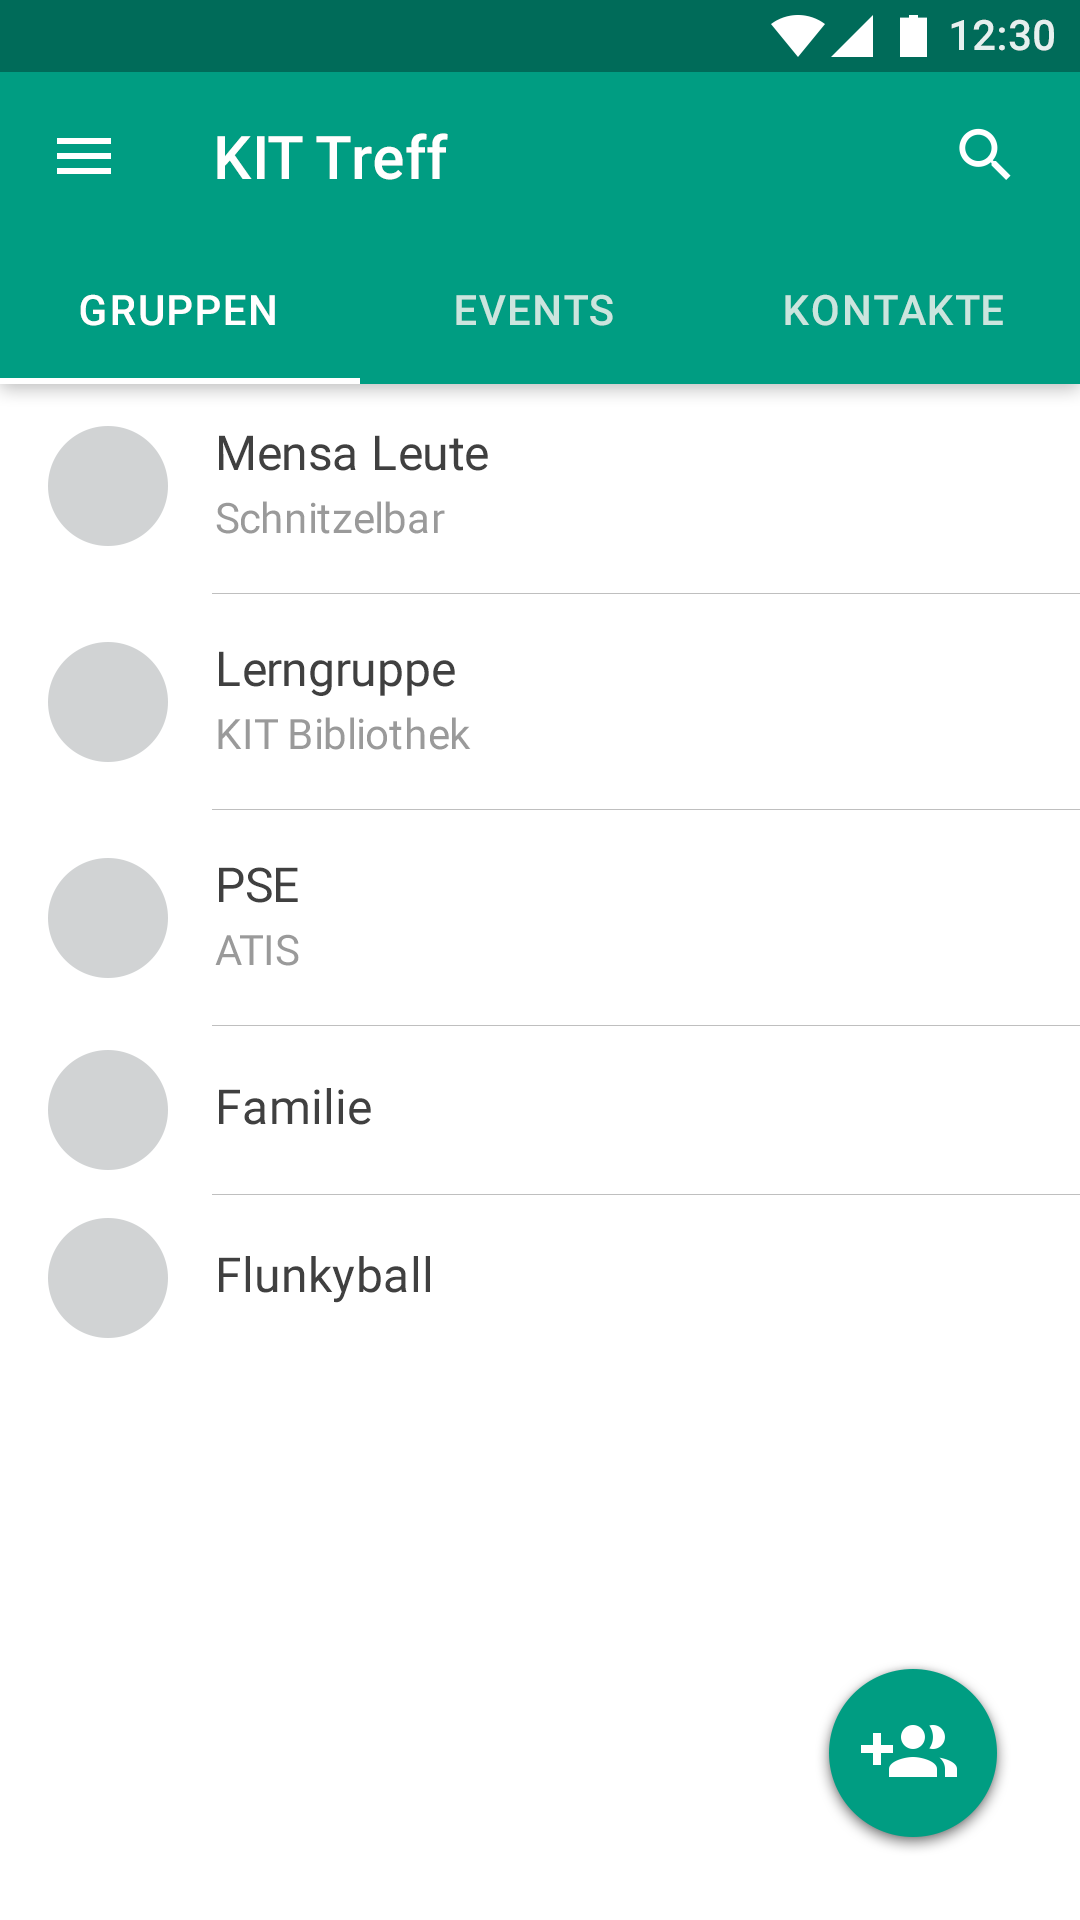
\includegraphics[height=80mm]{mockups/home_groups.png}}
	\caption{\label{fig:groups}
		Hier können Gruppen verwaltet und angesehen, sowie neue hinzugefügt werden.
		\testLink{grpcreate}.
			%TODO: test case
	}
\end{figure}

\begin{figure}[hb]
		\fbox{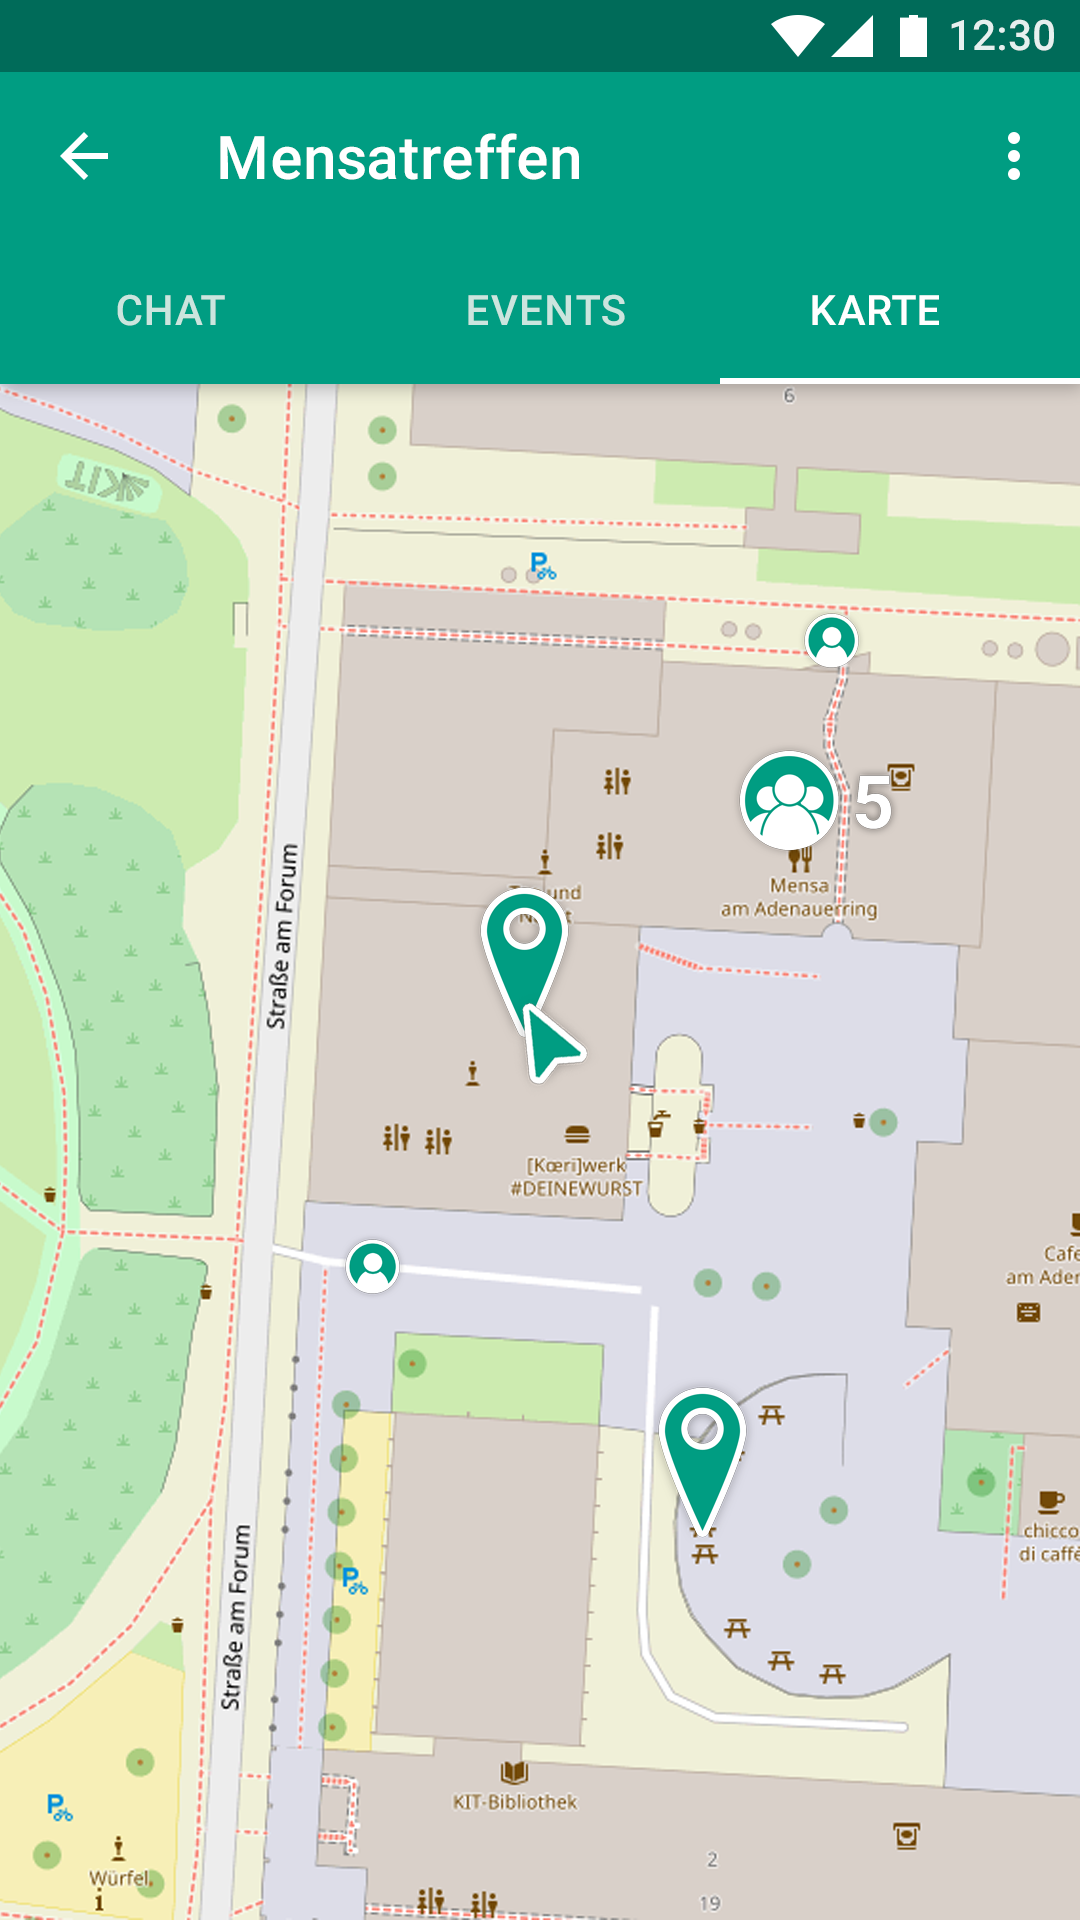
\includegraphics[height=80mm]{mockups/group_map.png}}
		\caption{\label{fig:map}
			Auf der Karte können die Positionen der anderen Gruppenmitglieder und bevorstehende
			Treffpunkte eingesehen werden. Nutzer erscheinen ggf. gruppiert.
			\testLink{grpcreate}.
			%TODO: test case
		}
\end{figure}

\begin{figure}[hb]
		\fbox{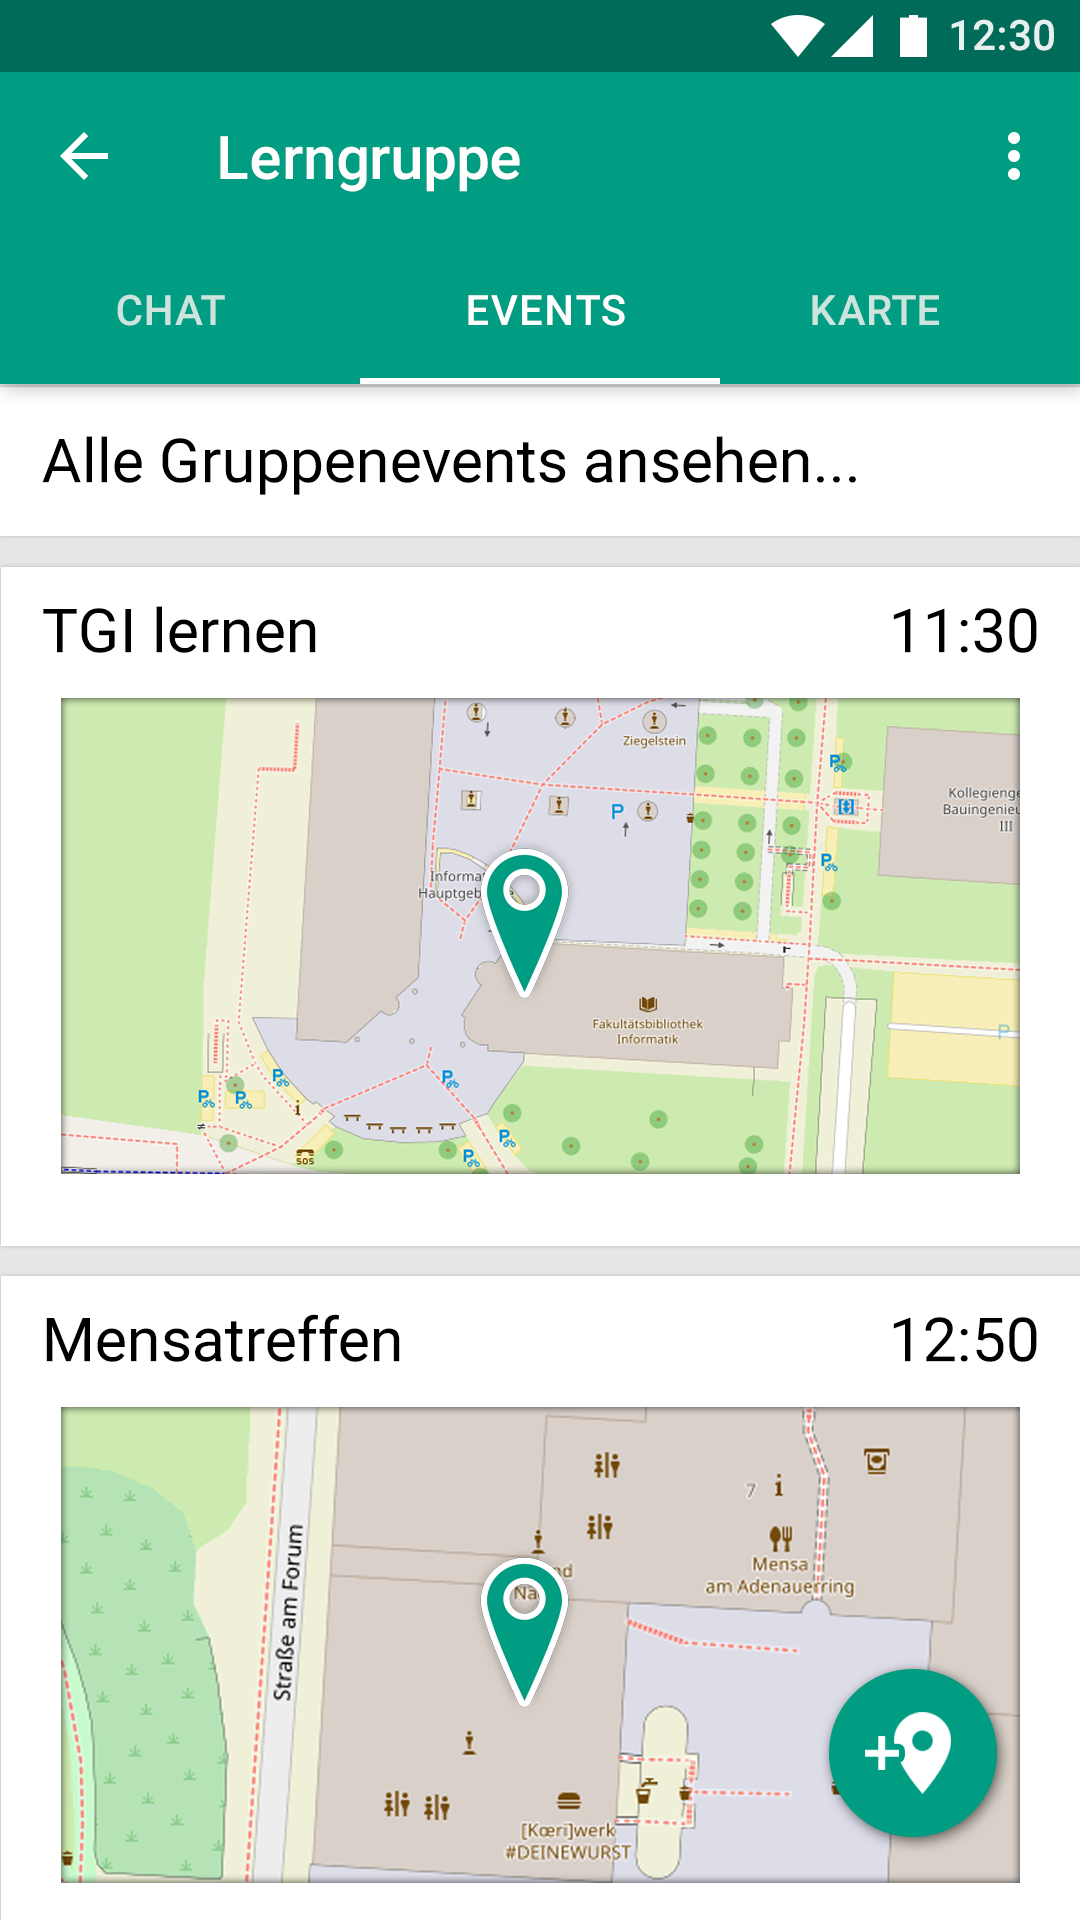
\includegraphics[height=80mm]{mockups/group_events.png}}
		\caption{\label{fig:map}
			Innerhalb der Gruppe können Treffpunkte eingesehen und hinzugefügt werden.
			\testLink{grpcreate}.
			%TODO: test case
		}
\end{figure}

\begin{figure}[hb]
		\fbox{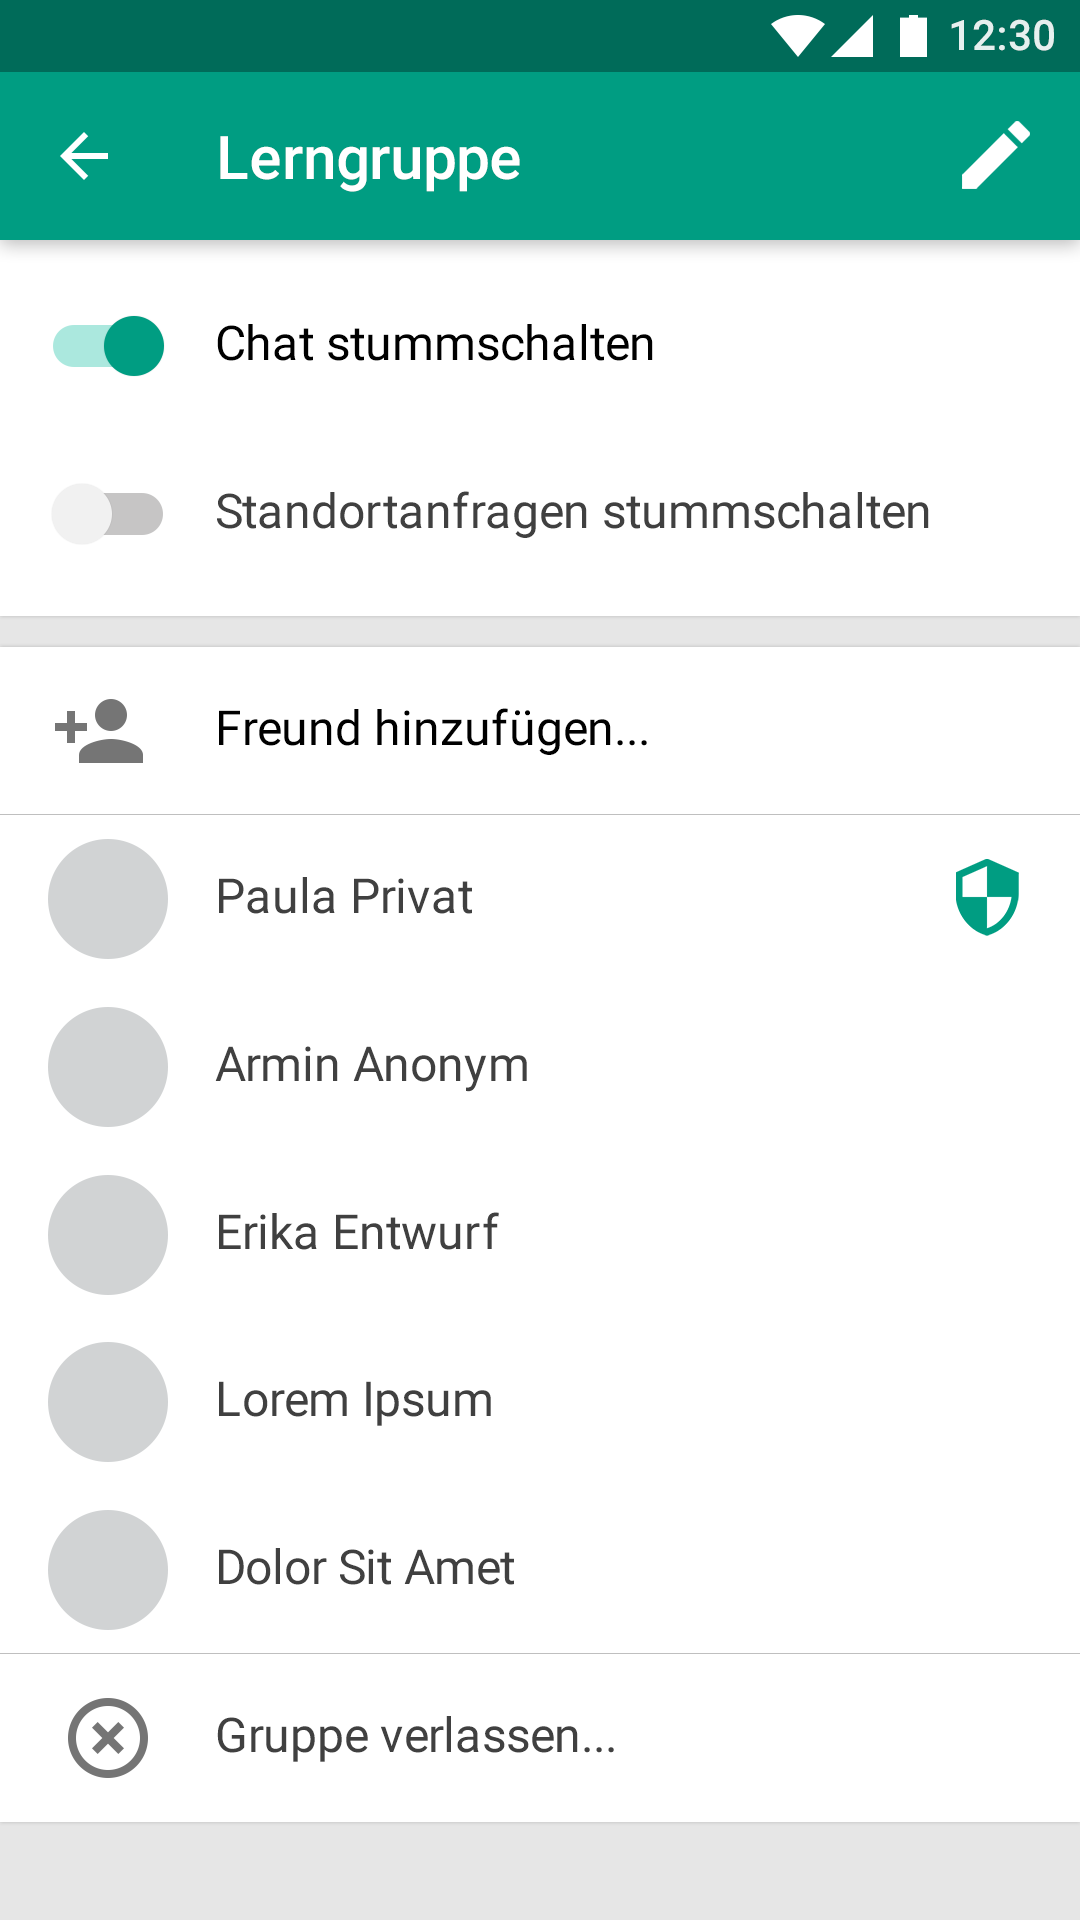
\includegraphics[height=80mm]{mockups/group_members.png}}
		\caption{\label{fig:map}
			Gruppenmitglieder können eingesehen, entfernt und hinzugefügt werden.
			Es gibt gruppenspezifische Einstellungsmöglichkeiten, sowie die Option,
			die Gruppe zu verlassen.
			\testLink{grpcreate}.
			%TODO: test case
		}
\end{figure}

\begin{figure}[hb]
		\fbox{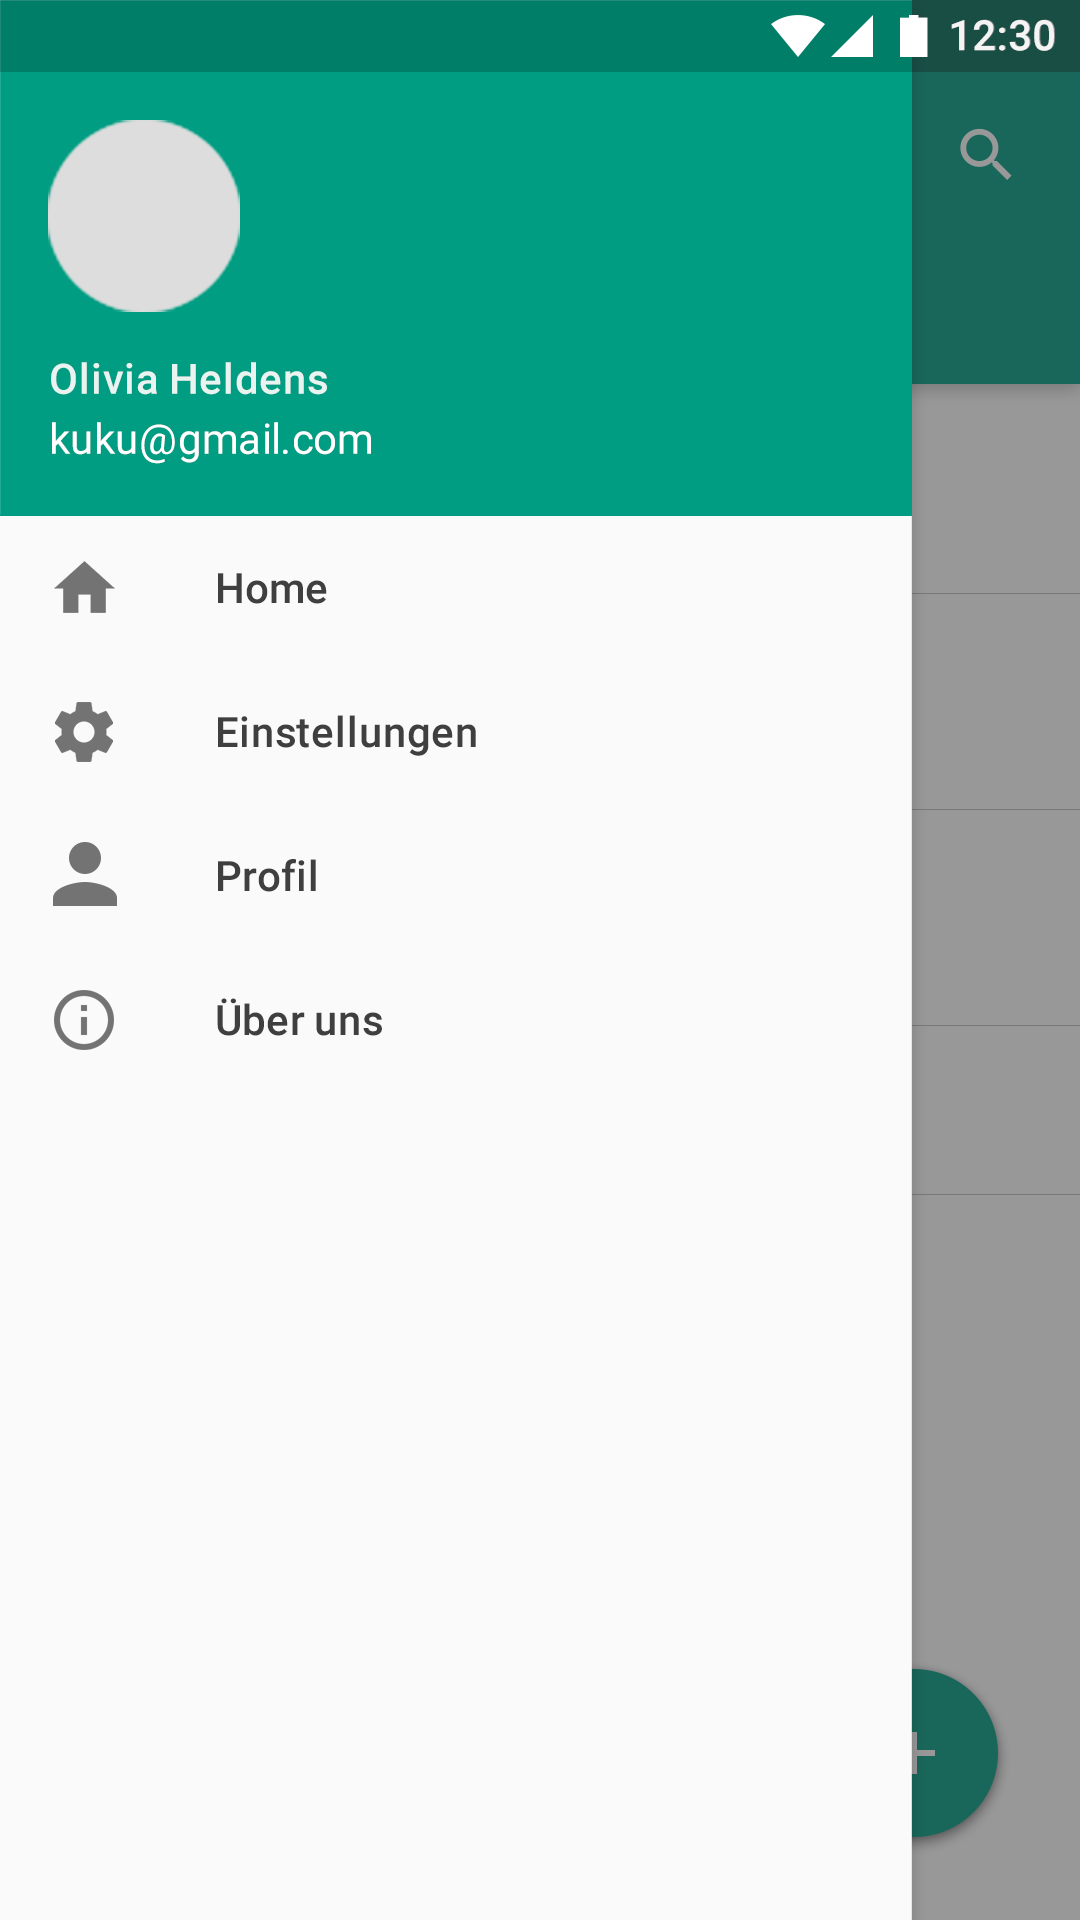
\includegraphics[height=80mm]{mockups/home_groups_sidenav.png}}
		\caption{\label{fig:map}
			Vom Startbildschirm aus können diverse Einstellungen erreicht werden.
			\testLink{grpcreate}.
			%TODO: test case
		}
\end{figure}

\section{Glossar}

\textbf{Nutzer}:
Ein eingeloggter Verwender der App.

\textbf{Gruppe}:
Mehrere Nutzer, welche untereinander Positionsdaten austauschen können.

\textbf{Chat}:
Möglichkeit für Mitglieder einer Gruppe, Textnachrichten auszutauschen.

\textbf{Verabredung}:
Ein festgelegter Ort und Zeitpunkt.

\textbf{Karte}:
Zeigt neben den kontextabhängigen Informationen der App auch Straßen, Gebäude und Terrain an.

\textbf{GPS}:
Global Positioning System, ein globales Satellitensystem zur Positionsbestimmung.

\end{document}
